\documentclass[ignorenonframetext,]{beamer}
\setbeamertemplate{caption}[numbered]
\setbeamertemplate{caption label separator}{: }
\setbeamercolor{caption name}{fg=normal text.fg}
\beamertemplatenavigationsymbolsempty
\usepackage{lmodern}
\usepackage{amssymb,amsmath}
\usepackage{ifxetex,ifluatex}
\usepackage{fixltx2e} % provides \textsubscript
\ifnum 0\ifxetex 1\fi\ifluatex 1\fi=0 % if pdftex
  \usepackage[T1]{fontenc}
  \usepackage[utf8]{inputenc}
\else % if luatex or xelatex
  \ifxetex
    \usepackage{mathspec}
  \else
    \usepackage{fontspec}
  \fi
  \defaultfontfeatures{Ligatures=TeX,Scale=MatchLowercase}
\fi
\usetheme[]{EastLansing}
\usecolortheme{crane}
\usefonttheme{structurebold}
% use upquote if available, for straight quotes in verbatim environments
\IfFileExists{upquote.sty}{\usepackage{upquote}}{}
% use microtype if available
\IfFileExists{microtype.sty}{%
\usepackage{microtype}
\UseMicrotypeSet[protrusion]{basicmath} % disable protrusion for tt fonts
}{}
\newif\ifbibliography
\hypersetup{
            pdftitle={MT4113, Computing in Statistics},
            pdfauthor={Lecture 2 - Algorithms to functions},
            pdfborder={0 0 0},
            breaklinks=true}
\urlstyle{same}  % don't use monospace font for urls
\usepackage{color}
\usepackage{fancyvrb}
\newcommand{\VerbBar}{|}
\newcommand{\VERB}{\Verb[commandchars=\\\{\}]}
\DefineVerbatimEnvironment{Highlighting}{Verbatim}{commandchars=\\\{\}}
% Add ',fontsize=\small' for more characters per line
\usepackage{framed}
\definecolor{shadecolor}{RGB}{248,248,248}
\newenvironment{Shaded}{\begin{snugshade}}{\end{snugshade}}
\newcommand{\KeywordTok}[1]{\textcolor[rgb]{0.13,0.29,0.53}{\textbf{#1}}}
\newcommand{\DataTypeTok}[1]{\textcolor[rgb]{0.13,0.29,0.53}{#1}}
\newcommand{\DecValTok}[1]{\textcolor[rgb]{0.00,0.00,0.81}{#1}}
\newcommand{\BaseNTok}[1]{\textcolor[rgb]{0.00,0.00,0.81}{#1}}
\newcommand{\FloatTok}[1]{\textcolor[rgb]{0.00,0.00,0.81}{#1}}
\newcommand{\ConstantTok}[1]{\textcolor[rgb]{0.00,0.00,0.00}{#1}}
\newcommand{\CharTok}[1]{\textcolor[rgb]{0.31,0.60,0.02}{#1}}
\newcommand{\SpecialCharTok}[1]{\textcolor[rgb]{0.00,0.00,0.00}{#1}}
\newcommand{\StringTok}[1]{\textcolor[rgb]{0.31,0.60,0.02}{#1}}
\newcommand{\VerbatimStringTok}[1]{\textcolor[rgb]{0.31,0.60,0.02}{#1}}
\newcommand{\SpecialStringTok}[1]{\textcolor[rgb]{0.31,0.60,0.02}{#1}}
\newcommand{\ImportTok}[1]{#1}
\newcommand{\CommentTok}[1]{\textcolor[rgb]{0.56,0.35,0.01}{\textit{#1}}}
\newcommand{\DocumentationTok}[1]{\textcolor[rgb]{0.56,0.35,0.01}{\textbf{\textit{#1}}}}
\newcommand{\AnnotationTok}[1]{\textcolor[rgb]{0.56,0.35,0.01}{\textbf{\textit{#1}}}}
\newcommand{\CommentVarTok}[1]{\textcolor[rgb]{0.56,0.35,0.01}{\textbf{\textit{#1}}}}
\newcommand{\OtherTok}[1]{\textcolor[rgb]{0.56,0.35,0.01}{#1}}
\newcommand{\FunctionTok}[1]{\textcolor[rgb]{0.00,0.00,0.00}{#1}}
\newcommand{\VariableTok}[1]{\textcolor[rgb]{0.00,0.00,0.00}{#1}}
\newcommand{\ControlFlowTok}[1]{\textcolor[rgb]{0.13,0.29,0.53}{\textbf{#1}}}
\newcommand{\OperatorTok}[1]{\textcolor[rgb]{0.81,0.36,0.00}{\textbf{#1}}}
\newcommand{\BuiltInTok}[1]{#1}
\newcommand{\ExtensionTok}[1]{#1}
\newcommand{\PreprocessorTok}[1]{\textcolor[rgb]{0.56,0.35,0.01}{\textit{#1}}}
\newcommand{\AttributeTok}[1]{\textcolor[rgb]{0.77,0.63,0.00}{#1}}
\newcommand{\RegionMarkerTok}[1]{#1}
\newcommand{\InformationTok}[1]{\textcolor[rgb]{0.56,0.35,0.01}{\textbf{\textit{#1}}}}
\newcommand{\WarningTok}[1]{\textcolor[rgb]{0.56,0.35,0.01}{\textbf{\textit{#1}}}}
\newcommand{\AlertTok}[1]{\textcolor[rgb]{0.94,0.16,0.16}{#1}}
\newcommand{\ErrorTok}[1]{\textcolor[rgb]{0.64,0.00,0.00}{\textbf{#1}}}
\newcommand{\NormalTok}[1]{#1}
\usepackage{graphicx,grffile}
\makeatletter
\def\maxwidth{\ifdim\Gin@nat@width>\linewidth\linewidth\else\Gin@nat@width\fi}
\def\maxheight{\ifdim\Gin@nat@height>\textheight0.8\textheight\else\Gin@nat@height\fi}
\makeatother
% Scale images if necessary, so that they will not overflow the page
% margins by default, and it is still possible to overwrite the defaults
% using explicit options in \includegraphics[width, height, ...]{}
\setkeys{Gin}{width=\maxwidth,height=\maxheight,keepaspectratio}

% Prevent slide breaks in the middle of a paragraph:
\widowpenalties 1 10000
\raggedbottom

\AtBeginPart{
  \let\insertpartnumber\relax
  \let\partname\relax
  \frame{\partpage}
}
\AtBeginSection{
  \ifbibliography
  \else
    \let\insertsectionnumber\relax
    \let\sectionname\relax
    \frame{\sectionpage}
  \fi
}
\AtBeginSubsection{
  \let\insertsubsectionnumber\relax
  \let\subsectionname\relax
  \frame{\subsectionpage}
}

\setlength{\parindent}{0pt}
\setlength{\parskip}{6pt plus 2pt minus 1pt}
\setlength{\emergencystretch}{3em}  % prevent overfull lines
\providecommand{\tightlist}{%
  \setlength{\itemsep}{0pt}\setlength{\parskip}{0pt}}
\setcounter{secnumdepth}{0}

\title{MT4113, Computing in Statistics}
\author{Lecture 2 - Algorithms to functions}
\date{19 September 2018}

\begin{document}
\frame{\titlepage}

\begin{frame}
\tableofcontents[hideallsubsections]
\end{frame}

\begin{frame}

\end{frame}

\section{Algorithms}\label{algorithms}

\begin{frame}{What is an algorithm?}

\begin{itemize}[<+->]
\tightlist
\item
  Algorithm: an \emph{ordered} sequence of \emph{unambiguous} and
  well-defined instructions for \emph{performing some task} and
  \emph{halting} in finite time
\item
  Important features:

  \begin{itemize}[<+->]
  \tightlist
  \item
    an ordered sequence
  \item
    unambiguous and well defined instructions - each instruction is
    clear, do-able, and can be done without difficulty
  \item
    performs some task - algorithm needs to be \emph{complete}, with
    nothing left out
  \item
    halts in finite time - i.e., the algorithm needs to terminate
  \end{itemize}
\end{itemize}

\end{frame}

\begin{frame}[fragile]{Example algorithm}

\begin{itemize}[<+->]
\tightlist
\item
  Example algorithm
\end{itemize}

\begin{verbatim}
* Algorithm soft boiled egg *
Put water in pan.
When the water boils, turn over the egg timer.
When the timer has run out, turn off the heat.
Pour some cold water into the pan to cool the water.
Remove egg.
\end{verbatim}

\begin{itemize}[<+->]
\tightlist
\item
  What is wrong with this algorithm?
\end{itemize}

\end{frame}

\section{Some elements of algorithms}\label{some-elements-of-algorithms}

\begin{frame}[fragile]{Assignment and computation}

\begin{itemize}[<+->]
\tightlist
\item
  Assigning values to variables

  \begin{itemize}[<+->]
  \tightlist
  \item
    \texttt{Let\ x\ :=\ 1}
  \end{itemize}
\item
  Computation

  \begin{itemize}[<+->]
  \tightlist
  \item
    \texttt{x\ :=\ x\ *\ 2}
  \end{itemize}
\end{itemize}

\end{frame}

\begin{frame}[fragile]{Input and output}

\begin{itemize}[<+->]
\tightlist
\item
  Input

  \begin{itemize}[<+->]
  \tightlist
  \item
    Reading values from files
  \item
    Passing values in at the start of the algorithm

    \begin{itemize}[<+->]
    \tightlist
    \item
      e.g., \texttt{Algorithm\ cakemix\ (sweet\_tooth)}
    \item
      \texttt{sweet\_tooth} is a \emph{parameter}
    \end{itemize}
  \end{itemize}
\item
  Output

  \begin{itemize}[<+->]
  \tightlist
  \item
    Printing results on screen
  \item
    Saving results to file
  \end{itemize}
\end{itemize}

\end{frame}

\begin{frame}[fragile]{Control structures: conditional execution}

\begin{itemize}[<+->]
\item
  Conditional operations ask a true/false question and then select the
  next instruction based on the answer
\item
  Example:

\begin{verbatim}
* Algorithm cakemix (sweet_tooth) *
In a bowl mix together:
  8 oz butter
  4 medium eggs
  2tsp vanilla extract
  8 oz self raising flour
  if (sweet_tooth) then
    8 oz caster sugar
  else
    4 oz caster sugar
  end if
  ...
\end{verbatim}
\end{itemize}

\end{frame}

\begin{frame}[fragile]{Control structures: iteration}

\begin{itemize}[<+->]
\item
  Iteration (looping): used to repeat a set of instructions
\item
  \textbf{Number of iterations known at outset} - example:

\begin{verbatim}
* Algorithm scramble (n) *
Do these statements n times:
  take an egg out of the fridge;
  crack the egg's shell on the edge of the bowl;
  pull the egg apart above the bowl;
  let the contents of the egg fall into the bowl;
  put the egg shell into the bin.
Stir egg conetnts in the bowl.
Pour contents of bowl into the frying pan.
...
\end{verbatim}
\item
  Notice the way indenting has been used to group commands together.
  Numbering could also be used (1.1, 1.2, etc.)
\end{itemize}

\end{frame}

\begin{frame}[fragile]

\begin{itemize}[<+->]
\item
  \textbf{Number of iterations not known at outset} (i.e., using a
  conditional operation to control the number of times a loop is
  executed).
\item
  Example:

\begin{verbatim}
* Algorithm cup of water *
...
Do these statements until the water level is on the line:
  If the level is above the line pour a little water out;
  If the level is below the line pour a little water in;
...
\end{verbatim}
\item
  Warning - potential for an infinite loop!

  \begin{itemize}[<+->]
  \tightlist
  \item
    Turn exact test into a ``good enough'' test -- see Lecture 4
  \item
    Add a stated limit on the number of iterations -- see Optimziation
    lectures
  \end{itemize}
\end{itemize}

\end{frame}

\begin{frame}[fragile]{Recursion}

\begin{itemize}[<+->]
\item
  Recursion: algorithms that call themselves.
\item
  Example:

\begin{verbatim}
* Algorithm factorial (n) *
If n == 1 then factorial = 1
  Else factorial = n * factorial(n - 1)
\end{verbatim}
\end{itemize}

\end{frame}

\section{Code and Pseudocode}\label{code-and-pseudocode}

\begin{frame}{What is code?}

\begin{itemize}[<+->]
\tightlist
\item
  Code: instructions in a computer language that implement an algorithm.
\end{itemize}

\end{frame}

\begin{frame}[fragile]

\begin{itemize}[<+->]
\tightlist
\item
  Example: factorial program in \texttt{R}
\end{itemize}

\begin{Shaded}
\begin{Highlighting}[]
\NormalTok{my.factorial <-}\StringTok{ }\ControlFlowTok{function}\NormalTok{(n) \{}
  \ControlFlowTok{if}\NormalTok{ (n }\OperatorTok{==}\StringTok{ }\DecValTok{1}\NormalTok{) \{}
    \KeywordTok{return}\NormalTok{(}\DecValTok{1}\NormalTok{)}
\NormalTok{  \} }\ControlFlowTok{else}\NormalTok{ \{}
    \KeywordTok{return}\NormalTok{(n }\OperatorTok{*}\StringTok{ }\KeywordTok{my.factorial}\NormalTok{ (n}\OperatorTok{-}\DecValTok{1}\NormalTok{))}
\NormalTok{  \}}
\NormalTok{\}}
\end{Highlighting}
\end{Shaded}

\begin{itemize}[<+->]
\tightlist
\item
  What's wrong with this function?
\end{itemize}

\end{frame}

\begin{frame}[fragile]{What is pseudocode?}

\begin{itemize}[<+->]
\item
  Pseudocode: instructions in a generic, informal, unspecified computer
  language that specify an algorithm.
\item
  Example - \texttt{Algorithm\ factorial\ (n)}
\item
  Tip: for anything other than completely trivial tasks, write out
  pseudocode on paper before writing any code on the computer!

  \begin{itemize}[<+->]
  \tightlist
  \item
    (For more on this, see next lecture)
  \end{itemize}
\end{itemize}

\end{frame}

\section{Control structures in R}\label{control-structures-in-r}

\begin{frame}[fragile]{Conditional execution}

\begin{itemize}[<+->]
\tightlist
\item
  Single condition
\end{itemize}

\begin{Shaded}
\begin{Highlighting}[]
\ControlFlowTok{if}\NormalTok{ (x }\OperatorTok{<}\StringTok{ }\DecValTok{10}\NormalTok{) y <-}\StringTok{ }\DecValTok{44}
\end{Highlighting}
\end{Shaded}

\end{frame}

\begin{frame}[fragile]

\begin{itemize}[<+->]
\tightlist
\item
  Multiple conditions
\end{itemize}

\begin{Shaded}
\begin{Highlighting}[]
\ControlFlowTok{if}\NormalTok{ ((x }\OperatorTok{<}\StringTok{ }\DecValTok{10}\NormalTok{)}\OperatorTok{|}\NormalTok{(y }\OperatorTok{>=}\StringTok{ }\DecValTok{12}\NormalTok{)) z <-}\StringTok{ }\DecValTok{44}
\end{Highlighting}
\end{Shaded}

\begin{Shaded}
\begin{Highlighting}[]
\ControlFlowTok{if}\NormalTok{ ((x }\OperatorTok{<}\StringTok{ }\DecValTok{10}\NormalTok{)}\OperatorTok{&}\NormalTok{(y }\OperatorTok{>=}\StringTok{ }\DecValTok{12}\NormalTok{)) z <-}\StringTok{ }\DecValTok{44}
\end{Highlighting}
\end{Shaded}

\end{frame}

\begin{frame}[fragile]

\begin{itemize}[<+->]
\tightlist
\item
  Two alternative outcomes
\end{itemize}

\begin{Shaded}
\begin{Highlighting}[]
\ControlFlowTok{if}\NormalTok{ (x }\OperatorTok{<}\StringTok{ }\DecValTok{10}\NormalTok{) \{}
\NormalTok{  y <-}\StringTok{ }\DecValTok{44}
\NormalTok{\} }\ControlFlowTok{else}\NormalTok{ \{}
\NormalTok{  z <-}\StringTok{ }\DecValTok{44}
\NormalTok{\}}
\end{Highlighting}
\end{Shaded}

\end{frame}

\begin{frame}[fragile]

\begin{itemize}[<+->]
\tightlist
\item
  Multiple alternative outcomes for the same variable
\end{itemize}

\begin{Shaded}
\begin{Highlighting}[]
\NormalTok{today <-}\StringTok{ "Wednesday"}
\NormalTok{event.}\DecValTok{4113}\NormalTok{ <-}\StringTok{ }\ControlFlowTok{switch}\NormalTok{(today,}
                \StringTok{"Monday"}\NormalTok{ =}\StringTok{ "lecture if week number is odd"}\NormalTok{,}
                \StringTok{"Tuesday"}\NormalTok{ =}\StringTok{ "frantic revision"}\NormalTok{,}
                \StringTok{"Wednesday"}\NormalTok{ =}\StringTok{ "thrilling lecture"}\NormalTok{,}
                \StringTok{"Thursday"}\NormalTok{ =}\StringTok{ "frantic revision"}\NormalTok{,}
                \StringTok{"Friday"}\NormalTok{ =}\StringTok{ "exciting practical"}\NormalTok{)}
\KeywordTok{print}\NormalTok{(}\KeywordTok{paste}\NormalTok{(today, }\StringTok{"will hold in store"}\NormalTok{, event.}\DecValTok{4113}\NormalTok{))}
\end{Highlighting}
\end{Shaded}

\begin{verbatim}
## [1] "Wednesday will hold in store thrilling lecture"
\end{verbatim}

\end{frame}

\begin{frame}[fragile]

\begin{itemize}[<+->]
\tightlist
\item
  Multiple alternative outcomes via nested conditional statements - more
  flexible but less elegant
\end{itemize}

\begin{Shaded}
\begin{Highlighting}[]
\ControlFlowTok{if}\NormalTok{ (x }\OperatorTok{<}\StringTok{ }\DecValTok{10}\NormalTok{) \{}
\NormalTok{  y <-}\StringTok{ }\DecValTok{44}
\NormalTok{\} }\ControlFlowTok{else}\NormalTok{ \{}
  \ControlFlowTok{if}\NormalTok{ (p }\OperatorTok{==}\StringTok{ }\DecValTok{14}\NormalTok{) \{}
\NormalTok{    z <-}\StringTok{ }\DecValTok{44}
\NormalTok{  \} }\ControlFlowTok{else}\NormalTok{ \{}
\NormalTok{    y <-}\StringTok{ }\NormalTok{x }\OperatorTok{+}\StringTok{ }\NormalTok{a}
\NormalTok{    today <-}\StringTok{ "Wednesday"}
\NormalTok{  \}}
\NormalTok{\}}
\end{Highlighting}
\end{Shaded}

\end{frame}

\begin{frame}[fragile]{Iteration (loops) - number of iterations known at
outset}

\begin{Shaded}
\begin{Highlighting}[]
\ControlFlowTok{for}\NormalTok{ (i }\ControlFlowTok{in} \DecValTok{1}\OperatorTok{:}\DecValTok{10}\NormalTok{) \{}
\NormalTok{  x[i] <-}\StringTok{ }\NormalTok{x[i] }\OperatorTok{*}\StringTok{ }\NormalTok{pi}
\NormalTok{\}}
\end{Highlighting}
\end{Shaded}

(Note - in many cases such loops can be vectorized.)

\end{frame}

\begin{frame}[fragile]{Iteration - number of iterations unknown at
outset}

While loop:

\begin{Shaded}
\begin{Highlighting}[]
\ControlFlowTok{while}\NormalTok{ (i }\OperatorTok{<}\StringTok{ }\DecValTok{27}\NormalTok{) \{}
\NormalTok{  x[i] <-}\StringTok{ }\NormalTok{x[i] }\OperatorTok{*}\StringTok{ }\NormalTok{pi}
\NormalTok{\}}
\end{Highlighting}
\end{Shaded}

Repeat until loop:

\begin{Shaded}
\begin{Highlighting}[]
\ControlFlowTok{repeat}\NormalTok{ \{ }
\NormalTok{  x[i] <-}\StringTok{ }\NormalTok{x[i] }\OperatorTok{*}\StringTok{ }\NormalTok{pi}
  \ControlFlowTok{if}\NormalTok{ (i }\OperatorTok{>=}\StringTok{ }\DecValTok{27}\NormalTok{) }\ControlFlowTok{break}
\NormalTok{\}}
\end{Highlighting}
\end{Shaded}

What is the difference between these?

\end{frame}

\begin{frame}[fragile]{Vectorization}

\begin{itemize}[<+->]
\tightlist
\item
  Many operations in \texttt{R} can be vectorized - these run much
  faster than loops
\end{itemize}

\begin{Shaded}
\begin{Highlighting}[]
\NormalTok{n<-}\FloatTok{1E8}
\NormalTok{x <-}\StringTok{ }\KeywordTok{rnorm}\NormalTok{(n)}
\KeywordTok{system.time}\NormalTok{(}
  \ControlFlowTok{for}\NormalTok{ (i }\ControlFlowTok{in} \DecValTok{1}\OperatorTok{:}\NormalTok{n) \{}
\NormalTok{    x[i] <-}\StringTok{ }\NormalTok{x[i] }\OperatorTok{*}\StringTok{ }\NormalTok{pi}
\NormalTok{  \}}
\NormalTok{)}
\end{Highlighting}
\end{Shaded}

\begin{verbatim}
## user system elapsed
## 14.18 0.03 14.33
\end{verbatim}

\end{frame}

\begin{frame}[fragile]

\begin{Shaded}
\begin{Highlighting}[]
\NormalTok{n<-}\FloatTok{1E8}
\NormalTok{x <-}\StringTok{ }\KeywordTok{rnorm}\NormalTok{(n)}
\KeywordTok{system.time}\NormalTok{(}
\NormalTok{  x <-}\StringTok{ }\NormalTok{x }\OperatorTok{*}\StringTok{ }\NormalTok{pi}
\NormalTok{)}
\end{Highlighting}
\end{Shaded}

\begin{verbatim}
## user system elapsed
## 0.16 0.05 0.21
\end{verbatim}

\end{frame}

\begin{frame}[fragile]

\textbf{The \texttt{apply} family of functions}

\begin{itemize}[<+->]
\tightlist
\item
  If data organized into data frames or matrices
\item
  You often need to iterate across colums or rows of the data
\end{itemize}

\begin{Shaded}
\begin{Highlighting}[]
\KeywordTok{data}\NormalTok{(iris3)}
\KeywordTok{apply}\NormalTok{(}\DataTypeTok{X =}\NormalTok{ iris3, }\DataTypeTok{MARGIN =} \DecValTok{2}\NormalTok{, }\DataTypeTok{FUN =}\NormalTok{ mean)}
\end{Highlighting}
\end{Shaded}

\begin{verbatim}
## Sepal L. Sepal W. Petal L. Petal W. 
## 5.843333 3.057333 3.758000 1.199333
\end{verbatim}

\begin{itemize}[<+->]
\tightlist
\item
  There are several variants of \texttt{apply} - \texttt{sapply},
  \texttt{lapply}, \texttt{tapply}, \texttt{mapply}, \texttt{\%by\%}
\item
  See, e.g., Matloff (2011) Sections 5.2 and 5.4 (esp 5.4.2)
\item
  Vectorization in \texttt{R} takes some getting used to - but
  persistence pays off!
\end{itemize}

\end{frame}

\section{Modular programming}\label{modular-programming}

\begin{frame}{what is ``modular programming''?}

Splittling a program into discrete, reuseable blocks of code so that
each block does a small amount.

\end{frame}

\begin{frame}[fragile]{Motivation}

Convert \texttt{-99} to \texttt{NA} in a dataset, of which this is a
fraction

\begin{verbatim}
##    a   b   c   d   e f
## 1  6   7   2   5   2 4
## 2  1   8 -99 -99 -99 6
## 3  1   5   9   5 -99 4
## 4  6 -99   9   6   1 1
## 5  9   8   6   1   8 9
## 6 10   7   9   9   5 5
\end{verbatim}

\end{frame}

\begin{frame}[fragile]

\begin{Shaded}
\begin{Highlighting}[]
\NormalTok{df}\OperatorTok{$}\NormalTok{a[df}\OperatorTok{$}\NormalTok{a }\OperatorTok{==}\StringTok{ }\OperatorTok{-}\DecValTok{99}\NormalTok{] <-}\StringTok{ }\OtherTok{NA}
\NormalTok{df}\OperatorTok{$}\NormalTok{b[df}\OperatorTok{$}\NormalTok{b }\OperatorTok{==}\StringTok{ }\OperatorTok{-}\DecValTok{99}\NormalTok{] <-}\StringTok{ }\OtherTok{NA}
\NormalTok{df}\OperatorTok{$}\NormalTok{c[df}\OperatorTok{$}\NormalTok{c }\OperatorTok{==}\StringTok{ }\OperatorTok{-}\DecValTok{98}\NormalTok{] <-}\StringTok{ }\OtherTok{NA}
\NormalTok{df}\OperatorTok{$}\NormalTok{d[df}\OperatorTok{$}\NormalTok{d }\OperatorTok{==}\StringTok{ }\OperatorTok{-}\DecValTok{99}\NormalTok{] <-}\StringTok{ }\OtherTok{NA}
\NormalTok{df}\OperatorTok{$}\NormalTok{e[df}\OperatorTok{$}\NormalTok{e }\OperatorTok{==}\StringTok{ }\OperatorTok{-}\DecValTok{99}\NormalTok{] <-}\StringTok{ }\OtherTok{NA}
\NormalTok{df}\OperatorTok{$}\NormalTok{f[df}\OperatorTok{$}\NormalTok{g }\OperatorTok{==}\StringTok{ }\OperatorTok{-}\DecValTok{99}\NormalTok{] <-}\StringTok{ }\OtherTok{NA}
\NormalTok{df}
\end{Highlighting}
\end{Shaded}

\begin{verbatim}
##    a  b   c  d  e f
## 1  6  7   2  5  2 4
## 2  1  8 -99 NA NA 6
## 3  1  5   9  5 NA 4
## 4  6 NA   9  6  1 1
## 5  9  8   6  1  8 9
## 6 10  7   9  9  5 5
\end{verbatim}

What happened?

\end{frame}

\begin{frame}[fragile]

\begin{itemize}[<+->]
\tightlist
\item
  Functions are the \texttt{R} way to implement modular programming
\end{itemize}

\begin{Shaded}
\begin{Highlighting}[]
\NormalTok{fix.missing <-}\StringTok{ }\ControlFlowTok{function}\NormalTok{(x) \{}
\NormalTok{  x[x }\OperatorTok{==}\StringTok{ }\OperatorTok{-}\DecValTok{99}\NormalTok{] <-}\StringTok{ }\OtherTok{NA}
  \KeywordTok{return}\NormalTok{(x)}
\NormalTok{\}}
\end{Highlighting}
\end{Shaded}

\begin{Shaded}
\begin{Highlighting}[]
\NormalTok{df}\OperatorTok{$}\NormalTok{a <-}\StringTok{ }\KeywordTok{fix.missing}\NormalTok{(df}\OperatorTok{$}\NormalTok{a)}
\NormalTok{df}\OperatorTok{$}\NormalTok{b <-}\StringTok{ }\KeywordTok{fix.missing}\NormalTok{(df}\OperatorTok{$}\NormalTok{b)}
\NormalTok{df}\OperatorTok{$}\NormalTok{c <-}\StringTok{ }\KeywordTok{fix.missing}\NormalTok{(df}\OperatorTok{$}\NormalTok{c)}
\NormalTok{df}\OperatorTok{$}\NormalTok{d <-}\StringTok{ }\KeywordTok{fix.missing}\NormalTok{(df}\OperatorTok{$}\NormalTok{d)}
\NormalTok{df}\OperatorTok{$}\NormalTok{e <-}\StringTok{ }\KeywordTok{fix.missing}\NormalTok{(df}\OperatorTok{$}\NormalTok{e)}
\NormalTok{df}\OperatorTok{$}\NormalTok{f <-}\StringTok{ }\KeywordTok{fix.missing}\NormalTok{(df}\OperatorTok{$}\NormalTok{e)}
\end{Highlighting}
\end{Shaded}

\begin{itemize}[<+->]
\tightlist
\item
  Still too much redundant code

  \begin{itemize}[<+->]
  \tightlist
  \item
    DRY principle

    \begin{itemize}[<+->]
    \tightlist
    \item
      Don't Repeat Yourself
    \end{itemize}
  \end{itemize}
\end{itemize}

\end{frame}

\begin{frame}[fragile]

\begin{itemize}[<+->]
\tightlist
\item
  Make use of inherent vectorisation in R
\end{itemize}

\begin{Shaded}
\begin{Highlighting}[]
\KeywordTok{fix.missing}\NormalTok{(df)}
\end{Highlighting}
\end{Shaded}

\begin{verbatim}
##    a  b  c  d  e f
## 1  6  7  2  5  2 4
## 2  1  8 NA NA NA 6
## 3  1  5  9  5 NA 4
## 4  6 NA  9  6  1 1
## 5  9  8  6  1  8 9
## 6 10  7  9  9  5 5
\end{verbatim}

\end{frame}

\begin{frame}[fragile]{Modules in R}

\begin{itemize}[<+->]
\tightlist
\item
  In \texttt{R}, modular programming is implemented through the use of
  \textbf{functions}
\item
  Syntax:
\end{itemize}

\begin{Shaded}
\begin{Highlighting}[]
\NormalTok{function.name <-}\StringTok{ }\ControlFlowTok{function}\NormalTok{(arguments) \{}
\NormalTok{  body}
\NormalTok{\}}
\end{Highlighting}
\end{Shaded}

\end{frame}

\begin{frame}[fragile]{Example R function}

\begin{itemize}[<+->]
\tightlist
\item
  Exploratory data analysis function - shows 3 plots and returns a
  summary of data vector \texttt{x}
\end{itemize}

\begin{Shaded}
\begin{Highlighting}[]
\NormalTok{eda <-}\StringTok{ }\ControlFlowTok{function}\NormalTok{ (x) \{}
  \KeywordTok{par}\NormalTok{(}\DataTypeTok{mfrow =} \KeywordTok{c}\NormalTok{(}\DecValTok{1}\NormalTok{ ,}\DecValTok{3}\NormalTok{))}
  \KeywordTok{hist}\NormalTok{(x, }\DataTypeTok{probability =} \OtherTok{TRUE}\NormalTok{)}
  \KeywordTok{lines}\NormalTok{(}\KeywordTok{density}\NormalTok{(x))}
  \KeywordTok{boxplot}\NormalTok{(x, }\DataTypeTok{horizontal =} \OtherTok{TRUE}\NormalTok{)}
  \KeywordTok{rug}\NormalTok{(x)}
  \KeywordTok{qqnorm}\NormalTok{(x)}
  \KeywordTok{return}\NormalTok{(}\KeywordTok{summary}\NormalTok{(x))}
\NormalTok{\}}
\end{Highlighting}
\end{Shaded}

\begin{itemize}[<+->]
\tightlist
\item
  (N.B. There are a few ``bad'' things about this function -- see next
  lecture for what!)
\end{itemize}

\end{frame}

\begin{frame}[fragile]

\begin{Shaded}
\begin{Highlighting}[]
\NormalTok{x <-}\StringTok{ }\KeywordTok{rnorm}\NormalTok{(}\DecValTok{100}\NormalTok{)}
\KeywordTok{eda}\NormalTok{(x)}
\end{Highlighting}
\end{Shaded}

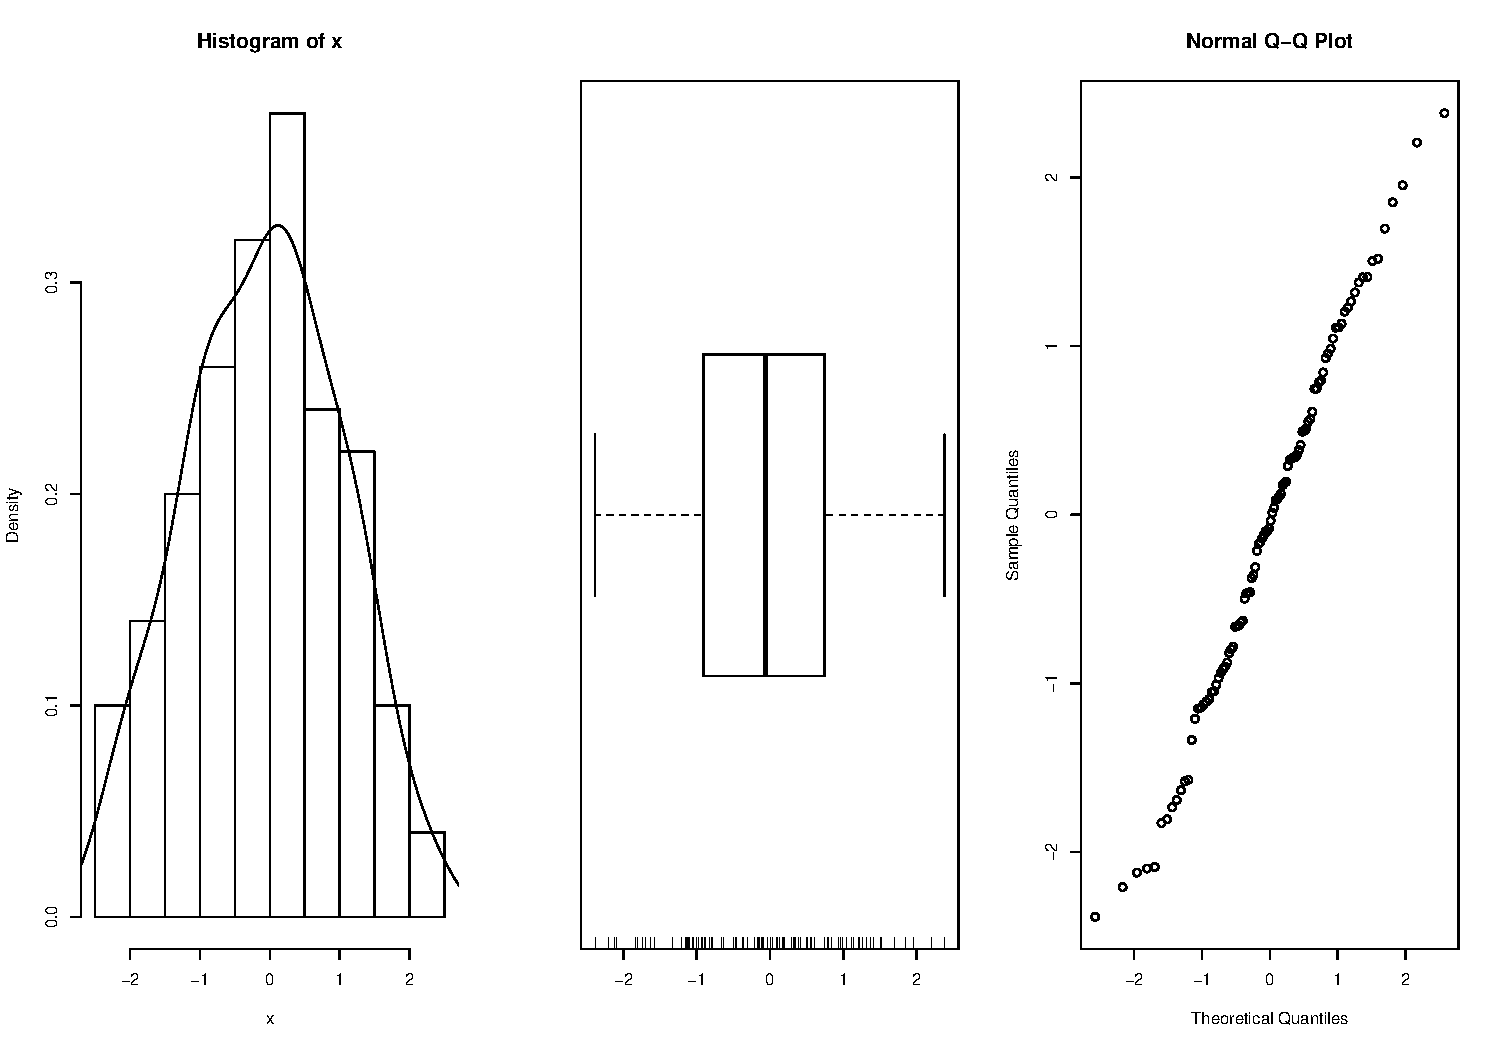
\includegraphics{lect2_files/figure-beamer/unnamed-chunk-22-1.pdf}

\begin{verbatim}
##     Min.  1st Qu.   Median     Mean  3rd Qu.     Max. 
## -2.38533 -0.90395 -0.05898 -0.07779  0.74749  2.38104
\end{verbatim}

\end{frame}

\begin{frame}[fragile]{Module interfaces - passing information in}

\begin{itemize}[<+->]
\tightlist
\item
  In general programmer-speak, the things you pass into modules are
  called ``parameters''
\item
  In `R they are called ``arguments''
\item
  E.g., in
\end{itemize}

\begin{Shaded}
\begin{Highlighting}[]
\NormalTok{print.and.multiply <-}\StringTok{ }\ControlFlowTok{function}\NormalTok{ (x, y) \{}
    \KeywordTok{cat}\NormalTok{(}\StringTok{'Inside function x='}\NormalTok{, x, }\StringTok{'y='}\NormalTok{, y, }\StringTok{'}\CharTok{\textbackslash{}n}\StringTok{'}\NormalTok{)}
    \KeywordTok{return}\NormalTok{(x }\OperatorTok{*}\StringTok{ }\NormalTok{y)}
\NormalTok{\}}
\end{Highlighting}
\end{Shaded}

\begin{itemize}[<+->]
\tightlist
\item
  \texttt{x} and \texttt{y} are function arguments
\end{itemize}

\end{frame}

\begin{frame}[fragile]

\begin{Shaded}
\begin{Highlighting}[]
\NormalTok{print.and.multiply <-}\StringTok{ }\ControlFlowTok{function}\NormalTok{ (x, y) \{}
    \KeywordTok{cat}\NormalTok{(}\StringTok{'Inside function x='}\NormalTok{, x, }\StringTok{'y='}\NormalTok{, y, }\StringTok{'}\CharTok{\textbackslash{}n}\StringTok{'}\NormalTok{)}
    \KeywordTok{return}\NormalTok{(x }\OperatorTok{*}\StringTok{ }\NormalTok{y)}
\NormalTok{\}}
\NormalTok{var.}\DecValTok{1}\NormalTok{ <-}\StringTok{ }\DecValTok{10}
\NormalTok{var.}\DecValTok{2}\NormalTok{ <-}\StringTok{ }\DecValTok{20}
\KeywordTok{print.and.multiply}\NormalTok{(var.}\DecValTok{1}\NormalTok{, var.}\DecValTok{2}\NormalTok{)}
\end{Highlighting}
\end{Shaded}

\begin{verbatim}
## Inside function x= 10 y= 20
\end{verbatim}

\begin{verbatim}
## [1] 200
\end{verbatim}

\end{frame}

\begin{frame}

\begin{itemize}[<+->]
\tightlist
\item
  In computer languages, there are two ways to make parameters
  (arguments) available to functions:

  \begin{itemize}[<+->]
  \tightlist
  \item
    passing by value
  \item
    passing by reference
  \end{itemize}
\end{itemize}

\end{frame}

\begin{frame}{Passing by value}

\begin{itemize}[<+->]
\tightlist
\item
  A copy is made of the value of each variable passed in to a function
\item
  These copies are stored in a separate location in memory from the
  original variables
\item
  So, changes to the variable inside the function have no affect on its'
  value outside the function
\end{itemize}

\end{frame}

\begin{frame}[fragile]

\begin{Shaded}
\begin{Highlighting}[]
\NormalTok{print.and.multiply <-}\StringTok{ }\ControlFlowTok{function}\NormalTok{ (x, y) \{}
    \KeywordTok{cat}\NormalTok{(}\StringTok{'Inside function x='}\NormalTok{, x, }\StringTok{'y='}\NormalTok{, y, }\StringTok{'}\CharTok{\textbackslash{}n}\StringTok{'}\NormalTok{)}
    \KeywordTok{return}\NormalTok{(x }\OperatorTok{*}\StringTok{ }\NormalTok{y)}
\NormalTok{\}}
\NormalTok{var.}\DecValTok{1}\NormalTok{ <-}\StringTok{ }\DecValTok{10}
\NormalTok{var.}\DecValTok{2}\NormalTok{ <-}\StringTok{ }\DecValTok{20}
\KeywordTok{print.and.multiply}\NormalTok{(var.}\DecValTok{1}\NormalTok{, var.}\DecValTok{2}\NormalTok{)}
\end{Highlighting}
\end{Shaded}

\begin{verbatim}
## Inside function x= 10 y= 20
\end{verbatim}

\begin{verbatim}
## [1] 200
\end{verbatim}

\begin{Shaded}
\begin{Highlighting}[]
\NormalTok{var.}\DecValTok{1}
\end{Highlighting}
\end{Shaded}

\begin{verbatim}
## [1] 10
\end{verbatim}

\begin{itemize}[<+->]
\tightlist
\item
  Aside - what would happen if you now typed \texttt{x}?
\end{itemize}

\end{frame}

\begin{frame}{Passing by reference}

\begin{itemize}[<+->]
\tightlist
\item
  The memory location of the variable passed in is given to the function
\item
  Therefore any changes to the variable within the function affect its'
  value after the function has completed
\item
  The following code will not work in R as it does not allow passing by
  reference:
\end{itemize}

\end{frame}

\begin{frame}[fragile]

\begin{verbatim}
print.and.multiply <- function (ByReference x, y) {
    cat('Inside function x=', x, 'y=', y, '\n')
    return(x * y)
}
var.1 <- 10
var.2 <- 20
print.and.multiply(var.1, var.2)
## [1] 200
var.1
## [1] 200
\end{verbatim}

\end{frame}

\begin{frame}{Pros and cons}

\begin{itemize}[<+->]
\tightlist
\item
  Passing by value

  \begin{itemize}[<+->]
  \tightlist
  \item
    Safer - you can do what you like with the variable inside the
    function, and you won't affect what goes on outside the function
  \item
    Inefficient - the computer has to make a copy of all variables -
    takes time and money
  \end{itemize}
\item
  Passing by reference

  \begin{itemize}[<+->]
  \tightlist
  \item
    Efficient - no copying of data
  \item
    Dangerous - anything you do to the variables inside the function
    affects their value outside
  \end{itemize}
\end{itemize}

\end{frame}

\begin{frame}[fragile]{Passing parameters - conclusion}

\begin{itemize}[<+->]
\tightlist
\item
  Most 3GLs let you choose which of the above is appropriate ot the
  circumstance
\item
  Some (e.g., C) allow you to specify whether variables passed by value
  can be changed within the function - best of both worlds!
\item
  Base \texttt{R} only supports passing by value
\item
  So how do you get information \textbf{out} of a function in
  \texttt{R}?

  \begin{itemize}[<+->]
  \tightlist
  \item
    Use \texttt{return} - see next section!
  \end{itemize}
\end{itemize}

\end{frame}

\begin{frame}[fragile]{Module interfaces - passing information out}

\begin{itemize}[<+->]
\tightlist
\item
  The main way to return values from functions is via the
  \texttt{return} statement
\end{itemize}

\begin{Shaded}
\begin{Highlighting}[]
\NormalTok{print.and.multiply <-}\StringTok{ }\ControlFlowTok{function}\NormalTok{ (x, y) \{}
    \KeywordTok{cat}\NormalTok{(}\StringTok{'Inside function x='}\NormalTok{, x, }\StringTok{'y='}\NormalTok{, y, }\StringTok{'}\CharTok{\textbackslash{}n}\StringTok{'}\NormalTok{)}
    \KeywordTok{return}\NormalTok{(x }\OperatorTok{*}\StringTok{ }\NormalTok{y)}
\NormalTok{\}}
\end{Highlighting}
\end{Shaded}

\begin{itemize}[<+->]
\tightlist
\item
  You can have more than one \texttt{return} statment (see factorial
  function earlier)
\end{itemize}

\end{frame}

\begin{frame}[fragile]

\begin{itemize}[<+->]
\tightlist
\item
  If you want to return more than one variable, use a named list
\end{itemize}

\begin{Shaded}
\begin{Highlighting}[]
\NormalTok{print.and.multiply <-}\StringTok{ }\ControlFlowTok{function}\NormalTok{ (x, y) \{}
    \KeywordTok{return}\NormalTok{(}\KeywordTok{list}\NormalTok{(}\DataTypeTok{x =}\NormalTok{ x, }\DataTypeTok{y =}\NormalTok{ y, }\DataTypeTok{mult =}\NormalTok{ x }\OperatorTok{*}\StringTok{ }\NormalTok{y))}
\NormalTok{\}}
\KeywordTok{print.and.multiply}\NormalTok{(}\DecValTok{10}\NormalTok{,}\DecValTok{20}\NormalTok{)}
\end{Highlighting}
\end{Shaded}

\begin{verbatim}
## $x
## [1] 10
## 
## $y
## [1] 20
## 
## $mult
## [1] 200
\end{verbatim}

\end{frame}

\begin{frame}[fragile]{Best practice for modular programming}

\begin{itemize}[<+->]
\tightlist
\item
  Pass everything requried by the function in as an argument
\item
  Pass everything out using a \texttt{return} statement
\item
  No global side effects
\item
  See next lecture for details, and many other tips for good programming
  practice\ldots{}
\end{itemize}

\end{frame}

\end{document}
